\documentclass[11pt]{article}
\usepackage[margin=0.85in]{geometry}
\usepackage{amsmath,amssymb,graphicx,booktabs,microtype}
\usepackage[round,authoryear]{natbib}
\usepackage[colorlinks=true,urlcolor=blue,citecolor=blue,linkcolor=blue]{hyperref}
\usepackage{float}
\usepackage{fancyhdr}
\pagestyle{fancy}
\fancyhf{}
\lhead{OpenJev: development report}
\rhead{September 2026}
\cfoot{\thepage}
\setlength{\headheight}{14pt}
\setlength{\parskip}{4pt}
\setlength{\parindent}{0pt}
\title{OpenJev: Bounded Decision Interfaces and a Bayesian Doom Control Pilot}
\author{OpenJev project\\\small\url{https://github.com/kw2828/OpenJev}}
\date{September 16, 2026\\\small Working research draft; not a conference submission}
\begin{document}
\maketitle
\begin{abstract}
OpenJev exposes request-defined questions and candidate answers as a typed decision interface, and uses those decisions to control a restricted Doom environment. We report three separate development measurements: a tiny imitation controller, a Bayesian firing-policy pilot, and a Rust/NumPy scoring-kernel comparison. In the valid 440-episode Bayesian study, posterior averaging did not establish a utility gain over the same logistic model's maximum a posteriori estimate. On the shifted scenario, mean utility was 5.140 versus 5.715, despite a descriptive improvement in shared-audit Brier score from 0.230733 to 0.226479. Conservative posterior gating reduced utility to 0.575. Separately, a 5,253-parameter imitation controller approximately matched its teacher over 20 paired seeds, while the median NumPy-to-Rust elapsed-time ratio was 2.70 in one local scoring-kernel microbenchmark. The study preserves a prior measurement failure and releases protocols, traces and plotting code. These results support further investigation of decision-aware information gathering; they do not establish a novel RL algorithm, calibrated action probabilities, or end-to-end acceleration.
\end{abstract}

\section{Motivation and scope}
A bounded application decision often needs a stable identifier and a score rather than generated prose. OpenJev accepts text context, a set of questions, and candidate identifiers with English descriptions. The application maps the returned identifier to an action. A pretrained Qwen language backend scores next-token candidate labels; it remains an autoregressive transformer and is not a new architecture. Questions are processed sequentially, without shared-prefix optimization.

The project is inspired by the typed-decision interface of Jev. It does not reproduce Jev's weights or proprietary Reinforcement Learning for Calibrated Decisions (RLCD). The research model in this report is a separate seven-feature Bayesian logistic outcome predictor. There is no language-model RL training, PPO, GRPO, or Bellman update in the pilot.

Our empirical question is narrow: \emph{does approximate Bayesian averaging or a conservative posterior bound improve firing decisions relative to the point estimate of the same learned model?} The original language-controller recording is a demonstration, not one of the fitted models or a baseline in this experiment.

\section{Decision interface and outcome model}
For candidate logits $z_1,\ldots,z_K$, the interface returns the conditional choice distribution
\begin{equation}
 q(a_i\mid c,Q,C)=\frac{\exp(z_i)}{\sum_{j=1}^{K}\exp(z_j)}.
\end{equation}
Here $c$ is context, $Q$ is the question, and $C$ is its candidate set. Candidate identifiers are preserved by the runtime. These uncalibrated scores sum to one but are not probabilities of task success. The runtime also reports candidate-label mass under the full vocabulary; restricting the denominator to candidates does not eliminate omitted-answer uncertainty.

The outcome model instead predicts a specified binary event when a fire command is issued. Let $x\in\mathbb{R}^7$ contain an intercept, visibility, clipped absolute aim error, target half-width, clipped distance, scaled health, and clipped ammo. With $y=1$ for a hit-count increase during the following seven game tics,
\begin{align}
 p(y=1\mid x,w)&=\sigma(x^\top w),\qquad w\sim\mathcal{N}(0,I),\\
 \hat w&=\arg\min_w\sum_n\left[\log(1+e^{x_n^\top w})-y_nx_n^\top w\right]+\tfrac12\lVert w\rVert^2,\\
 \Sigma&=\left[I+X^\top\operatorname{diag}(p_n(1-p_n))X\right]^{-1}.
\end{align}
Newton steps with line search fit the MAP estimate, with at most 40 iterations. A Laplace approximation uses $w\mid D\approx\mathcal{N}(\hat w,\Sigma)$. Twenty-node Gauss--Hermite quadrature approximates $\bar p(x)=\mathbb{E}_{w\mid D}[\sigma(x^\top w)]$. The lower probability used for conservative gating is
\begin{equation}
 p_{\rm low}(x)=\sigma\left(x^\top\hat w-1.645\sqrt{x^\top\Sigma x}\right).
\end{equation}
This is approximately a one-sided 95\% posterior lower bound conditional on the fitted approximation, not a conformal or frequentist coverage guarantee. The implementation separates $\operatorname{Var}_{w\mid D}(p)$ and $\mathbb{E}_{w\mid D}[p(1-p)]$. Neither decomposition corrects feature misspecification or temporal dependence.

The three learned policies issue fire when $p_{\rm MAP}$, $\bar p$, or $p_{\rm low}$ respectively exceeds the fixed threshold 0.25. This is a myopic decision rule; it does not account for future survival or information value. A negative Brier reward primitive is available in the package, but is \emph{not} the fitting loss used here.

\section{Experimental design and measurement}
We use ViZDoom \citep{kempka2016vizdoom}, with privileged visible-actor labels and game variables rather than pixels. Five independent collection seeds each produce 16 training episodes in Defend the Center. The behavior policy requests fire with probability 0.6 and randomizes steering with probability 0.2. Only issued fire-command windows provide outcome labels; cooldown windows without a hit count as failures. Waiting does not generate a synthetic negative label.

All five evaluated firing policies share rule-based steering. The comparisons are the existing rule, the tiny imitation model's firing output, logistic MAP, Bayesian mean, and Bayesian lower bound. Each learned policy is evaluated on ten paired seeds per scenario for each of five training replicates. The rule and imitation baselines are each run once per seed and reused in paired comparisons, not counted as independent copies. Evaluation seeds 40000--40009 are disjoint from fitting. Episodes have at most 180 seven-tic decisions, and there is no evaluation-time fitting or threshold tuning.

The 440 episodes comprise 80 training episodes, 20 common-audit episodes and 340 evaluation episodes. The common audit applies a randomized behavior policy to supply the same observed firing events to all fitted models. It has ten episodes per scenario, containing 349 center and 700 line events. These events are dependent within episodes and do not expose every counterfactual action outcome. Utility is
\begin{equation}
 U=\sum_{t:\,\text{issued fire}}(y_t-0.25).
\end{equation}
It measures command-window outcomes, not per-bullet accuracy or the default game reward. Intervals use 10,000 paired crossed-bootstrap resamples over five training replicates and ten evaluation seeds. They are exploratory, unadjusted intervals with small sampling units.

\paragraph{Preserved failed measurement.}
The preceding v1 run also completed 440 episodes, but used net ammo decrease to detect shots. Ammo replenishment in Defend the Line masked firing, causing zero detected shots and empty calibration audits. The original traces and quality exception are retained. V2 changes the estimand to commanded firing windows and uses fresh evaluation seeds; it is a new development study, not a repaired identical replication or sealed confirmation. Only v2 supports the cross-scenario tables here.

\section{Bayesian pilot results}
\begin{table}[H]
\centering\small
\begin{tabular}{lrrr}
\toprule
Controller & Center utility & Line utility & Line kills \\
\midrule
Rule baseline & 3.175 & 13.900 & 26.90 \\
Tiny imitation & 3.150 & 13.100 & 25.40 \\
Logistic MAP & 0.855 & 5.715 & 16.34 \\
Bayesian mean & 0.870 & 5.140 & 16.96 \\
Bayesian lower bound & 1.000 & 0.575 & 4.76 \\
\bottomrule
\end{tabular}

\caption{Mean v2 outcomes. Learned controllers have 50 evaluation episodes per scenario; each existing baseline has ten. All policies share rule steering. The table is generated directly from the preserved analysis JSON.}
\end{table}

Bayesian mean minus MAP utility was $+0.015$ in the center scenario (exploratory 95\% interval $[-0.705,0.725]$), and $-0.575$ in the line scenario ($[-3.745,1.960]$). These intervals do not establish a benefit, equivalence, or absence of smaller effects. The conservative lower bound performed worse in the line scenario: $-5.140$ relative to MAP ($[-9.120,-1.720]$). Strong rule and imitation baselines further limit any claim of learned-control progress.

\begin{figure}[H]
\centering
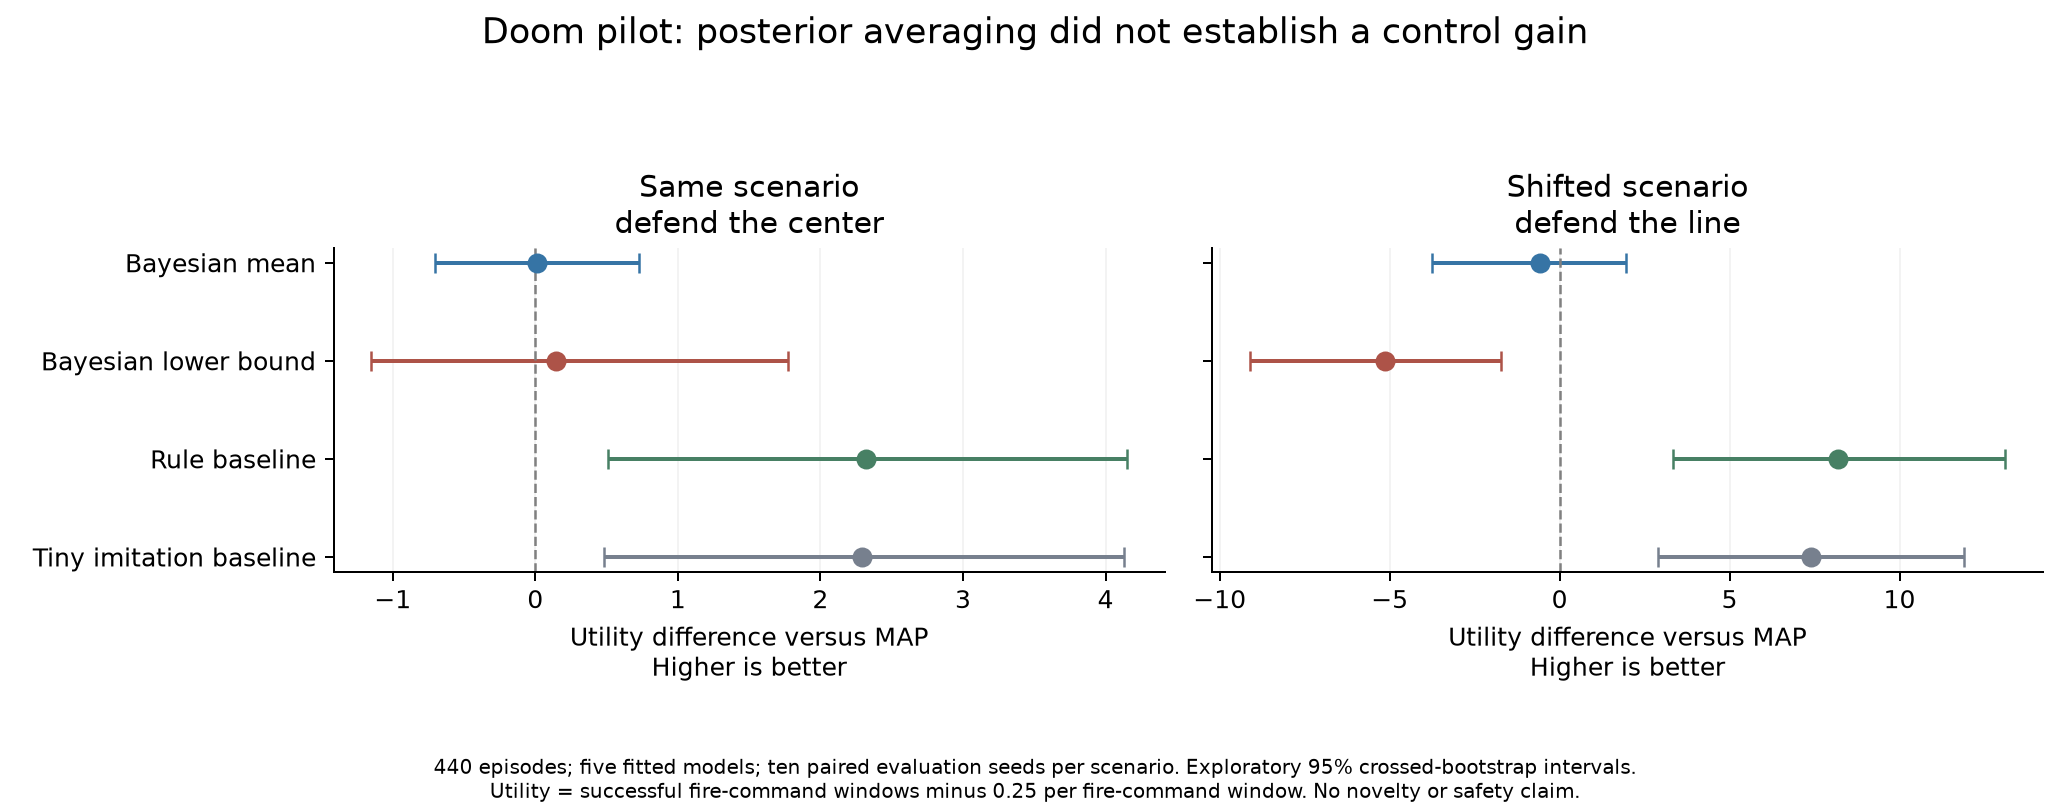
\includegraphics[width=\linewidth]{../evidence/bayesian-doom-v2/utility-comparison.png}
\caption{Paired utility differences from MAP. Positive values favor the compared controller. Intervals account for training replicate and episode-seed variation, but are exploratory and unadjusted.}
\end{figure}

\begin{figure}[H]
\centering
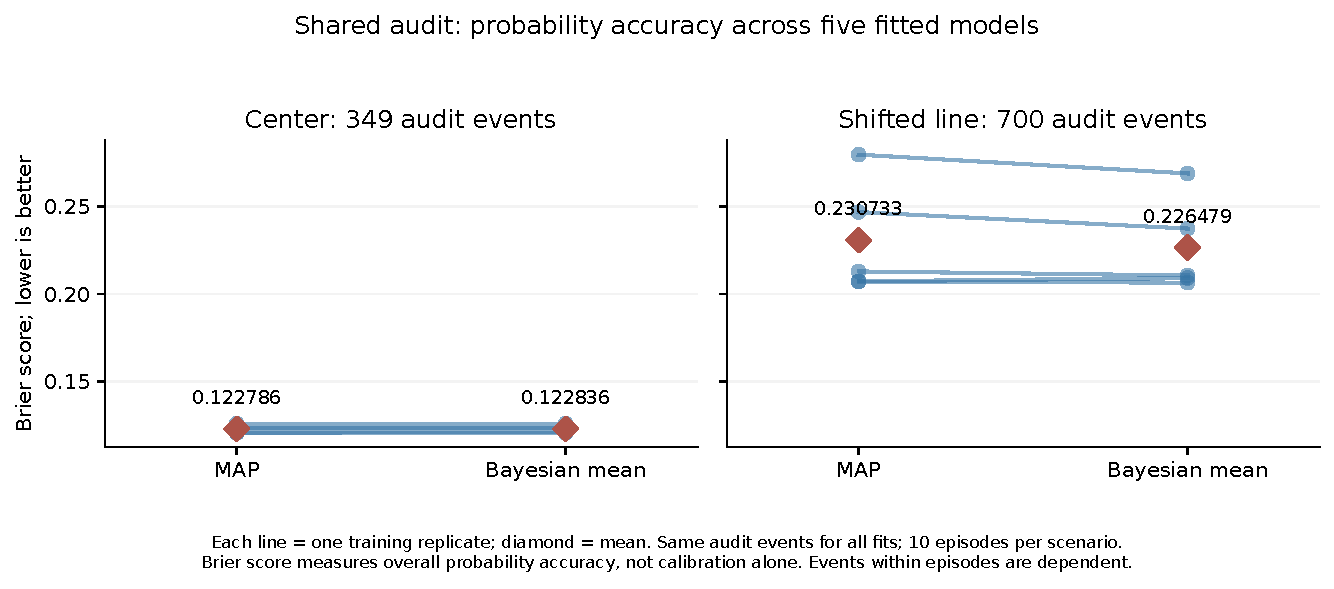
\includegraphics[width=.95\linewidth]{../evidence/benchmarks/audit-brier.pdf}
\caption{Paired audit Brier scores across five fitted models. The same events are reused across fits, so the five lines are not five independent audit datasets. Red diamonds are means, not confidence intervals.}
\end{figure}

On the shared line audit, the mean Brier score decreased descriptively from 0.230733 to 0.226479 with Bayesian averaging; in the center it changed from 0.122786 to 0.122836. Brier score measures overall probability accuracy and is not an isolated calibration diagnostic. No uncertainty interval is reported for this descriptive audit comparison. Its apparent improvement in the shifted scenario did not coincide with better mean control utility. This local result motivates measuring prediction and decision performance separately, rather than treating one as a substitute for the other.

\section{Separate gameplay and systems benchmarks}
\paragraph{Original imitation benchmark.}
The shipped 5,253-parameter MLP uses 11 numeric features and two 64-unit hidden layers, with separate steering and firing heads. It was trained on 60,000 synthetic states labeled by an explicit rule controller. On 20 matched center-scenario seeds (1000--1019), mean kills were 17.55 for imitation, 17.60 for the teacher, and 0.95 for random control. These runs use two-tic actions and complete steering policies. Their kill counts must not be merged with or directly ranked against the seven-tic firing-only Bayesian study.

\begin{figure}[H]
\centering
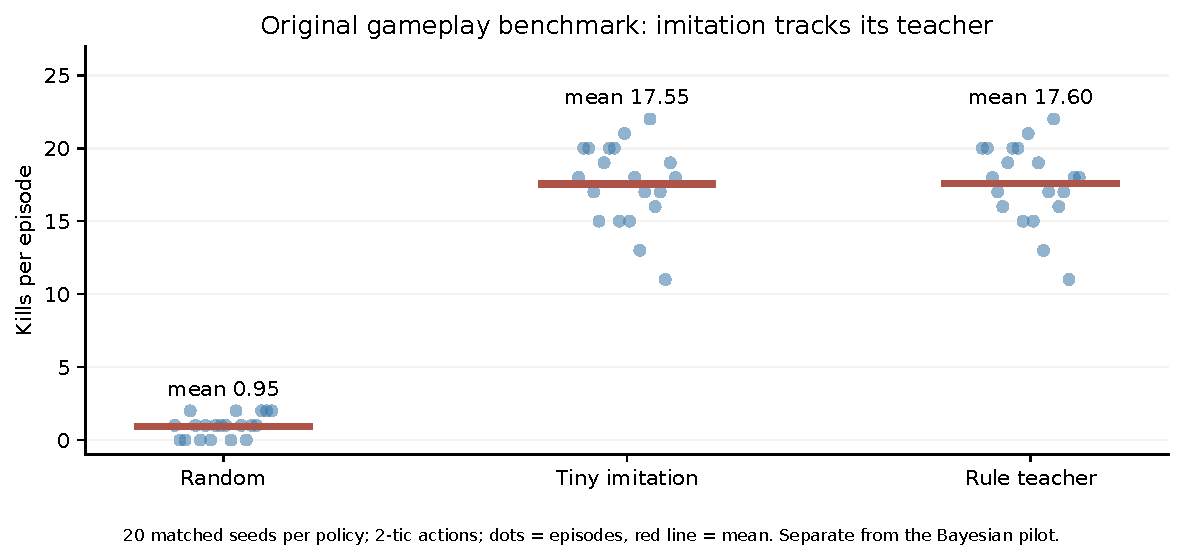
\includegraphics[width=.92\linewidth]{../evidence/benchmarks/gameplay.pdf}
\caption{All 60 episodes of the original gameplay benchmark. The imitation policy approximates its teacher on this scenario. This is not a generalization or superiority claim.}
\end{figure}

\paragraph{Rust versus NumPy score kernel.}
Both implementations receive identical float64 logits with 32 rows, vocabulary width 151,936 and six candidates. They compute candidate probabilities, full-vocabulary candidate mass, and entropy. Inputs include extreme and equal-valued rows. After three warmups, each implementation runs 11 timed batches. Maximum output difference is $1.11\times10^{-18}$. Median elapsed time per row was 0.550013 ms for Python/NumPy and 0.203807 ms for Rust release, giving a ratio of 2.699.

\begin{figure}[H]
\centering
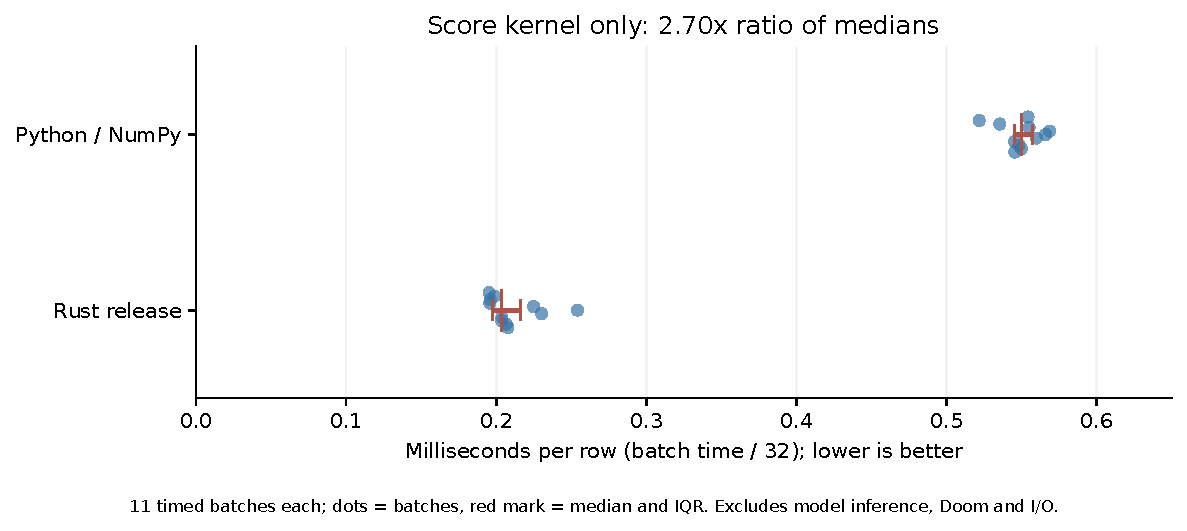
\includegraphics[width=.92\linewidth]{../evidence/benchmarks/score-kernel.pdf}
\caption{One local score-kernel microbenchmark: points are batch time divided by 32; red marks show medians and interquartile ranges, not confidence intervals. This excludes model inference, tokenization, Doom, HTTP, startup and I/O.}
\end{figure}

This measurement used Linux ARM64 in Docker with a two-CPU limit, Python 3.12.14, NumPy 2.5.3 and Rust 1.94.0. Rust ran before Python, and other Docker services remained active. NumPy already executes native numerical kernels, so the result compares these implementations, not interpreted arithmetic with compiled arithmetic. It is not evidence of a general Rust advantage or end-to-end agent acceleration. Randomized execution order, additional machines and end-to-end profiling remain necessary for stronger claims.

\section{Related work and limitations}
Calibration for learned dynamics and control is established research \citep{malik2019calibrated}. The Laplace approximation used here is also established \citep{daxberger2021laplace}; applying it to this logistic head is not a new Bayesian method. RLCR combines correctness and calibration rewards for reasoning language models \citep{damani2025beyond}. We do not train or reproduce RLCR, and its results cannot be transferred to our firing-policy experiment.

The pilot's linear features omit weapon cooldown and temporal state. Its conditional-independence likelihood ignores within-episode correlation, which may invalidate the posterior's uncertainty interpretation. The lower-bound policy may suppress useful firing, but this study does not isolate the mechanism. Two scenarios from one game, five training sets and ten evaluation seeds are insufficient to establish robust generality. Neither the eight disclosed language development questions nor a single gameplay GIF is an independent language benchmark. No evaluated connectome-inspired architecture, latent transformer, recurrent world model, semantic-entropy method or conformal decision guarantee is established by this report.

\section{Next hypothesis and reproducibility}
A follow-up should ask whether additional observations or recurrent computation improve the \emph{decision}, conditional on their cost. Forecast learning and action selection should remain separately measurable. A proposed controller would allocate extra work only when estimated decision improvement exceeds its cost, rather than using posterior width alone. This is a research hypothesis, not an implemented contribution in these results.

Required controls include the same head without Bayes, fixed extra computation, scalar probability and entropy gates, and matched-data/compute ensembles. Random audit actions need known propensities and support checks. Development and confirmation splits should be fixed before tuning, with a second environment and an English decision task. Literature review must establish a distinct method or theoretical result before any ICLR novelty claim.

The repository retains the v1 and v2 execution snapshots at commits \texttt{4007e64} and \texttt{f59ca5c}, frozen protocols, source hashes, episode summaries, posterior weights and losslessly compressed traces. Hashes of raw traces refer to decompressed bytes. V2 completed in 85.18 workstation seconds; this duration is not a portable throughput benchmark. All five fits had gradient norms below $8\times10^{-8}$ and positive covariance eigenvalues, validating numerical mechanics rather than model specification.

\texttt{research/plot\_benchmarks.py} regenerates the new figures and table from checked-in evidence and writes a source-hash manifest. The paper's build instructions distinguish regeneration of figures from rerunning experiments. The v1 quality exception remains visible; invalid cross-scenario observations are not pooled into v2. Code and artifacts are available at \url{https://github.com/kw2828/OpenJev}.

\bibliographystyle{plainnat}
\bibliography{references}
\end{document}
